% =====================================================================
% UNIVERSAL-BEISPIEL: ABBILDUNGEN IN LATEX (STABIL & UTF-8)
% Zeigt alle wichtigen Szenarien, die man in einer Diplomarbeit benötigt.
% =====================================================================

\documentclass[a4paper,12pt]{article} 
% Dokumentklasse 'article': Standard für Berichte, Hausarbeiten, Diplomarbeiten
% Papierformat: A4, Schriftgröße: 12pt

% ---------------------------------------------------------------------
% PAKETE (erweitern LaTeX um zusätzliche Funktionen)
% ---------------------------------------------------------------------
\usepackage[ngerman]{babel}        
% Aktiviert deutsche Sprache (Übersetzungen, Silbentrennung)

\usepackage{graphicx}              
% Ermöglicht das Einfügen von Bildern mit \includegraphics

\usepackage[labelfont=bf,font=small]{caption} 
% Gestaltet Bildunterschriften:
% - "Abbildung X" fett gedruckt
% - Text der Bildunterschrift in kleinerer Schriftgröße

\usepackage{subcaption}            
% Ermöglicht Unterabbildungen (mehrere Bilder in einer Figure-Umgebung)

\usepackage{float}                 
% Ermöglicht feste Positionierung mit [H] = „Hier und nicht woanders“

\usepackage{wrapfig}               
% Lässt Text um eine Grafik herumlaufen (Textumlauf)

\usepackage{rotating}              
% Zum Drehen von Objekten (z. B. Abbildungen um 90°)

\usepackage{pdfpages}              
% Zum Einfügen kompletter PDF-Seiten ins Dokument

\usepackage{geometry}              
% Zum Anpassen der Seitenränder (hier nicht explizit verändert)

\usepackage{csquotes}              
% Sorgt für korrekte deutsche Anführungszeichen („Text“)

% Eingabekodierung UTF-8
\usepackage[T1]{fontenc}

% Schriftkodierung T1 für korrekte Silbentrennung und Umlaute
\usepackage[ngerman]{babel}

% Deutsche Lokalisierung (Trennung, Bezeichnungen)
\usepackage{booktabs}

% booktabs für saubere horizontale Linien
\usepackage{tabularx}

% tabularx für flexible Spaltenbreiten (X-Spalten)
\usepackage{longtable}

% longtable für mehrseitige Tabellen
\usepackage{multirow}

% multirow für Zusammenführen von Zellen über mehrere Zeilen
\usepackage{siunitx}

% siunitx für saubere Zahlenausrichtung
\usepackage{caption}

% Farben für Code-Highlighting
\usepackage{xcolor}

% Für Codeblöcke
\usepackage{listings}

% Gibt den Ordner an, in dem sich die Bilder befinden (hier: ./images/)
\graphicspath{{images/}}           

% Kleine Schriftgröße für Bildunterschriften
\captionsetup{font=small}
 
% Listing Kopfzeile umbenennen
\renewcommand{\lstlistingname}{Codeblock}

% Farbschema
% Was soll eingefärbt werden | HTML Colorcode | HEX Code
\definecolor{codebg}{HTML}{F7F7F7}
\definecolor{codeframe}{HTML}{E0E0E0}
\definecolor{codekw}{HTML}{005CC5}
\definecolor{codestr}{HTML}{E36209}
\definecolor{codecom}{HTML}{6A737D}
\definecolor{codety}{HTML}{22863A}
\definecolor{codenum}{HTML}{111111}

% Neuen Code-Stil erstellen
\lstdefinestyle{cstyle}{ % Neuen Stil definieren
  language=C, % Sprache
  backgroundcolor=\color{codebg}, % Farbschema
  frame=single, % Rahmenoptionen
  rulecolor=\color{codeframe}, % Rahmenoptionen
  frameround=tttt, % Rahmenoptionen
  basicstyle=\ttfamily\small, % Monospace und kleiner
  numbers=left, % Zeilennummern auf der linken Seite
  numberstyle=\footnotesize\color{codenum}, % Stil der Nummern definieren
  stepnumber=1, % Schritte der Nummern
  numbersep=8pt, % Größe der Nummern
  showstringspaces=false, % Leerzeichen in Strings anzeigen
  tabsize=4, % Größe von Tabs in Leerzeichen
  keepspaces=true, % Leerzeichen verwenden
  breaklines=true, % Lange Zeichen umbrechen
  keywordstyle=\bfseries\color{codekw}, % Schlüsselwörter wie If While etc. in bestimmten Farbstil
  stringstyle=\color{codestr}, % Strings in bestimmten Farbstil
  commentstyle=\itshape\color{codecom}, % Kommentare in bestimmten Farbstil
  morekeywords={uint8_t,uint16_t,uint32_t,size_t,inline,bool}, % zusätzliche Typen
  emph={uint8_t,uint16_t,uint32_t,size_t,bool}, emphstyle=\color{codety}\bfseries
}

% Neuer Python-Code-Stil
\lstdefinestyle{pystyle}{ % Neuen Stil definieren
  language=Python, % Sprache
  backgroundcolor=\color{codebg}, % Hintergrundfarbe
  frame=single, % Rahmen um Codeblock
  rulecolor=\color{codeframe}, % Rahmenfarbe
  frameround=tttt, % abgerundete Ecken
  basicstyle=\ttfamily\small, % Monospace-Schrift, klein
  numbers=left, % Zeilennummern links
  numberstyle=\footnotesize\color{codenum}, % Stil der Nummern
  stepnumber=1, % Jede Zeile nummerieren
  numbersep=8pt, % Abstand Nummer ↔ Code
  showstringspaces=false, % Keine Markierung für Leerzeichen in Strings
  tabsize=4, % Tabweite in Leerzeichen
  keepspaces=true, % Leerzeichen beibehalten
  breaklines=true, % Lange Zeilen umbrechen
  keywordstyle=\bfseries\color{codekw}, % Schlüsselwörter (def, if, for, ...)
  stringstyle=\color{codestr}, % Strings ("..." oder '...')
  commentstyle=\itshape\color{codecom}, % Kommentare (# ...)
  emph={int,float,bool,list,dict,set,tuple,str,range,zip,enumerate}, emphstyle=\color{codety}\bfseries, % Typen/Objekte grün
  morekeywords={self,True,False,None,async,await,with,as,lambda,yield,from,import}, % Zusätzliche Schlüsselwörter
}

% ---------------------------------------------------------------------
% DOKUMENTMETADATEN
% ---------------------------------------------------------------------
\title{Code, Abbildungen und Tabellen einbinden, Minipages mit Text/Code/Abbildungen}
\author{Schönauer Simon, Zagler Fabian, Bachleitner-Huber Florian, Meinhart Manuel}
\date{\today}

% =====================================================================
\begin{document}

\maketitle
% Erstellt automatisch die Titelseite mit Titel, Autor und Datum

\newpage
% Erzwingt Seitenumbruch nach dem Inhaltsverzeichnis

% =====================================================================
%Zagler
% =====================================================================
\centering
\section{Code einbinden mit Listings}
{\large von Fabian Zagler}

\vspace{1 cm}

\begin{lstlisting}[style=cstyle, caption={Code Beispiel mit cstyle Stil}, label={lst:C}]
#include <stdio.h>

int fibonacci(int n) {
    if (n <= 1)
        return n;
    return fibonacci(n - 1) + fibonacci(n - 2);
}

int main(void) {
    int n = 10;

    printf("Fibonacci(%d) = %d\n", n, fibonacci(n));

    return 0;
}
\end{lstlisting}



\begin{lstlisting}[style=pystyle, captionpos=b, caption={Beispiel einer Fibonacci-Funktion in Python}, label={lst:py}]
def fibonacci(n):
    if n <= 1:
        return n
    return fibonacci(n - 1) + fibonacci(n - 2)

if __name__ == "__main__":
    n = 10
    print(f"Fibonacci({n}) = {fibonacci(n)}")
\end{lstlisting}


\vspace{1 cm}


\noindent
In Listing~\ref{lst:C} wird die Fibonacci-Funktion in C gezeigt.\\
In Listing~\ref{lst:py} wird die Fibonacci-Funktion in Python gezeigt.



\newpage

% =====================================================================
% Meinhart
% =====================================================================
\section{Einfache Minipage Beispiele}  % Hauptabschnitt
{\large von Manuel Meinhart}

\subsection{Minipages nebeneinander}   % Unterabschnitt
\noindent  % Verhindert Einrückung des folgenden Absatzes
\begin{figure}[!h]  % Floating-Umgebung für Bilder, !h = "here if possible"
    \centering      % Zentriert den Inhalt

    \begin{minipage}[t]{0.3\textwidth}
        \centering
        
\includegraphics[width=\textwidth]{Bild1.jpg}
        \caption{Bild links}
    \end{minipage}
    \begin{minipage}[t]{0.3\textwidth}
        \centering
        
\includegraphics[width=\textwidth]{Bild2.jpg}
        \caption{Bild Mitte}
    \end{minipage}
    \begin{minipage}[t]{0.3\textwidth}
        \centering
        
\includegraphics[width=\textwidth]{Bild3.jpg}
        \caption{Bild rechts}
    \end{minipage}
    \caption{Drei Bilder nebeneinander}
\end{figure}

\vspace{0.5 cm}

\begin{figure}[!h]
  \centering

  \begin{minipage}{0.45\textwidth}
    \centering
    \includegraphics[width=\linewidth]{example-image-a}
    \caption{Bild A}
    \label{fig:first}
  \end{minipage}
  \hfill
  \begin{minipage}{0.45\textwidth}
    \centering
    \includegraphics[width=\linewidth]{example-image-b}
    \caption{Bild B}
    \label{fig:second}
  \end{minipage}

  \caption{Zwei Bilder nebeneinander}
  \label{fig:both}
\end{figure}

\newpage

\subsection{Bild und Text nebeneinander}  % Unterabschnitt für Bild-Text-Kombination
\begin{figure}[!h]  % Neue Floating-Umgebung

  \centering  % Zentriert den gesamten Inhalt
  \begin{minipage}[b]{0.45\textwidth}  % Linke Minipage, 45% der Textbreite, am unteren Rand ausgerichtet
    \centering  % Zentriert den Inhalt der Minipage
    
\includegraphics[width=\textwidth]{Bild1.jpg}  % Bild mit voller Breite der Minipage
    \caption{Bild links}  % Bildunterschrift für linke Seite
  \end{minipage}
  \begin{minipage}[b]{0.45\textwidth}  % Rechte Minipage, 45% der Textbreite
    \raggedright  % Text linksbündig ausrichten
    % Beispieltext mit manuellen Zeilenumbrüchen
    Dies ist ein Beispieltext, der rechts neben dem Bild steht.\\
    Er kann mehrere Zeilen umfassen und erklärt das Bild.\\

    \vspace{0.8 cm}  % Vertikaler Abstand von 0.8cm

    In diesem Fall sehen wir ein schönes Laptop Hintergundbild.\\
    \caption{Text rechts}  % Bildunterschrift für rechte Seite
  \end{minipage}
\end{figure}
    
\subsection{Code und Text nebeneinander}  % Unterabschnitt für Code-Text-Kombination
\begin{figure}[!h]  % Neue Floating-Umgebung

  \centering  % Zentriert den gesamten Inhalt
  \begin{minipage}[b]{0.55\textwidth}  % Linke Minipage für Code, 55% der Textbreite
    \centering  % Zentriert den Inhalt der Minipage
    % Code-Block mit definiertem Stil
\begin{lstlisting}[style=cstyle]
#include <stdio.h>

int main(void) {
    printf("Hello, World!\n");
    return 0;
}
\end{lstlisting}
    \caption{Code links}  % Bildunterschrift für den Code
  \end{minipage}
  \begin{minipage}[b]{0.4\textwidth}  % Rechte Minipage für Text, 40% der Textbreite
    \centering  % Zentriert den Inhalt
    \begin{itemize}  % Aufzählungsliste
      \item Dies ist ein einfaches C-Programm.  % Erster Listenpunkt
      \item Es gibt "Hello, World!" auf der Konsole aus.  % Zweiter Listenpunkt
    \end{itemize}
    \caption{Text rechts}  % Bildunterschrift für den Text
  \end{minipage}
\end{figure}



\newpage

% =====================================================================
%Bachleitner
% =====================================================================
\section{Beispiele: Tabellenformate}
{\large von Florian Bachleitner-Huber}

\vspace{1 cm}

In diesem Dokument sind mehrere Möglichkeiten gezeigt, wie man Tabellen mit drei Spalten in LaTeX setzen kann. Zu jeder Tabelle gibt es eine kurze Erklärung.

\subsection*{1) Einfache linksbündige Tabelle}
% Beispiel 1: einfache linksbündige Tabelle
	\textit{Erklärung:} Standardtabular mit drei linksbündigen Spalten (l).	%beschreibt, dass hier eine Standarttabelle mit linksbündigen Spalten gezeigt wird.
\begin{table}[h!]															%erlaubt Latex Tabellen zu positionieren,h! heißt das es hundertprozentig hier erscheinen soll.
	\centering								                                %zentriert die Tabelle auf der Seite
	\caption{Einfache linksbündige Tabelle}                                 %Beschriftung der Tabelle
	\begin{tabular}{lll}                                                    %Tabellenumgebung mit 3 linken Spalten
	
		Spalte 1 & Spalte 2 & Spalte 3 \\                                   %Tabellenkopf
		\midrule                                                            %horizontale Linie
		A1 & A2 & A3 \\                                                     %erste Datenzeile
		B1 & B2 & B3 \\                                                     %zweite Datenzeile
		\bottomrule                                                         %horizontale Linie unten
	\end{tabular}                                                           %Ende der Tabellenumgebung
\end{table}                                                                 %Ende der Tabelle

\subsection*{2) Zentrierte und rechtsbündige Spalten}
% Beispiel 2: zentrierte und rechtsbündige Spalten
	\textit{Erklärung:} Verwende c für zentriert und r für rechtsbündig.
\begin{table}[h!]
	\centering
	\caption{Zentriert / Rechts}
	\begin{tabular}{crr}
	
		Spalte 1 & Spalte 2 & Spalte 3 \\
		\midrule
		Text & 123 & 4.56 \\
		Mehr & 78 & 9.10 \\
		\bottomrule
	\end{tabular}
\end{table}

\subsection*{3) Vertikale Linien}
% Beispiel 3: vertikale Linien in der Tabelle
	\textit{Erklärung:} Senkrechte Linien mit |; oft weniger empfohlen, aber in manchen Fällen gebraucht.
\begin{table}[h!]
	\centering
	\caption{Mit vertikalen Linien}
	\begin{tabular}{|l|c|r|}
		\hline
		Spalte 1 & Spalte 2 & Spalte 3 \\
		\hline
		A & B & C \\
		D & E & F \\
		\hline
	\end{tabular}
\end{table}

\subsection*{4) Feste Spaltenbreite mit p{width}}
% Beispiel 4: feste Spaltenbreite mit p{..}
	\textit{Erklärung:} p{<Breite>} erlaubt Textumbruch in Zellen.
\begin{table}[h!]
	\centering
	\caption{Feste Breite (p{4cm})}
	\begin{tabular}{p{4cm}p{4cm}p{4cm}}

		 Überschrift 1 &  Überschrift 2 &  Überschrift 3 \\
		\midrule
		Dies ist ein längerer Text, der umbrechen soll. & Kurz & Noch ein langer Text, der umbrechen wird. \\
		\bottomrule
	\end{tabular}
\end{table}

\subsection*{5) Flexible Breite mit tabularx}
% Beispiel 5: flexible Breite mit tabularx
	\textit{Erklärung:} \texttt{tabularx} mit X-Spalten verteilt die Breite automatisch.
\begin{table}[h!]
	\centering
	\caption{tabularx mit X-Spalten}
	\begin{tabularx}{\textwidth}{X X X}
		
		Überschrift 1 & Überschrift 2 & Überschrift 3 \\
		\midrule
		Text links & Mittel & Rechts \\
		Noch Text & Noch mehr & Und noch mehr \\
		\bottomrule
	\end{tabularx}
\end{table}

\subsection*{6) Tabellen mit booktabs}
% Beispiel 6: booktabs für saubere Linien
	\textit{Erklärung:} \texttt{booktabs} erzeugt professionellere horizontale Linien (toprule, midrule, bottomrule).
\begin{table}[h!]
	\centering
	\caption{booktabs Beispiel}
	\begin{tabular}{lll}
		
		Spalte A & Spalte B & Spalte C \\
		\midrule
		1 & 2 & 3 \\
		4 & 5 & 6 \\
		\bottomrule
	\end{tabular}
\end{table}

\newpage

\subsection*{7) Zahlen und Einheiten mit siunitx}
% Beispiel 7: Zahlenformatierung mit siunitx
	\textit{Erklärung:} \texttt{siunitx} formatiert Zahlen und Einheiten sauber; r-Alignment mit S-Spalten.
\begin{table}[h!]
	\centering
	\caption{siunitx Beispiel}
	\begin{tabular}{l S S}
	
		Messung & {Wert 1} & {Wert 2} \\
		\midrule
		Probe A & 1234.56 & 7.89 \\
		Probe B & 12.3 & 456.0 \\
		\bottomrule
	\end{tabular}
\end{table}

\subsection*{8) Mehrere Zeilen }
% Beispiel 8: multirow / multicolumn
	\textit{Erklärung:} \texttt{multirow} und \texttt{multicolumn} erlauben das Zusammenführen von Zellen.
	\begin{table}[h!]
	\centering
	\caption{multirow / multicolumn}
	\begin{tabular}{lll}
			\toprule
		& Spalte 2 & Spalte 3 \\
		\midrule
		\multirow{2}{*}{Gruppe 1} & A & B \\
		 & C & D \\
		\midrule
		\multicolumn{2}{c}{Zusammengefasst} & E \\
		\bottomrule
	\end{tabular}
\end{table}

\subsection*{9) Lange Tabellen über Seiten: longtable}
% Beispiel 9: longtable für mehre Seiten
	\textit{Erklärung:} \texttt{longtable} erlaubt Tabellen, die sich über mehrere Seiten erstrecken.
\begin{longtable}{lll}
	\caption{longtable Beispiel} \\
	\toprule
	Kopf 1 & Kopf 2 & Kopf 3 \\
	\midrule
	\endfirsthead
	\multicolumn{3}{c}{Fortsetzung von vorheriger Seite} \\
	\toprule
	Kopf 1 & Kopf 2 & Kopf 3 \\
	\midrule
	\endhead
	Ein & Zwei & Drei \\
	Eins & Zwei & Drei \\
	% (weitere Zeilen würden hier folgen)
	\bottomrule
\end{longtable}



\newpage
% =====================================================================
%Schönauer
% =====================================================================
\section{Abbildungen in LaTeX}
{\large von Simon Schönauer}

\vspace{1 cm}

\large Vollständige Referenz mit allen Szenarien
% =====================================================================
\subsection{Grundlagen und einfache Abbildungen}
% =====================================================================

\subsubsection{Einfache Abbildung mit verschiedenen Positionierungen}

\paragraph{Positionierung mit [H] (exakt hier)}
\begin{figure}[H]
  % [H] = Abbildung wird GENAU hier platziert (nicht verschieben!)
  % Benötigt das float-Paket
  \centering
  % Bild horizontal zentrieren
  
\includegraphics[width=0.6\textwidth]{BMW.jpg}
  % width=0.6\textwidth bedeutet: Breite = 60% der Textbreite
  \caption{Abbildung mit [H] wird genau hier platziert.}
  % Bildunterschrift unter dem Bild
  \label{fig:einfach-h}
  % Label für Referenzierung im Text (mit \ref{fig:einfach-h})
\end{figure}

\paragraph{Positionierung mit [htbp] (LaTeX entscheidet)}
\begin{figure}[htbp]
  % [htbp] = LaTeX entscheidet selbst die beste Position
  % h = here (hier bevorzugt)
  % t = top (oben auf der Seite)
  % b = bottom (unten auf der Seite)  
  % p = page (eigene Seite nur für Abbildungen)
  \centering
  
\includegraphics[width=0.6\textwidth]{BMW.jpg}
  \caption{Abbildung mit [htbp] wird von LaTeX optimal platziert.}
  \label{fig:einfach-htbp}
\end{figure}

\subsubsection{Referenzierung im Text}
% Mit \ref{label} wird die Abbildungsnummer eingefügt
% Mit \pageref{label} wird die Seitenzahl eingefügt
% ~ erzeugt ein geschütztes Leerzeichen (verhindert Zeilenumbruch)
Wie in Abbildung~\ref{fig:einfach-h} auf Seite~\pageref{fig:einfach-h} zu sehen ist, lassen sich Bilder leicht einfügen. Man kann auch auf Abbildung~\ref{fig:einfach-htbp} verweisen.

% =====================================================================
\subsection{Größenanpassung und Skalierung}
% Es gibt drei Hauptmethoden: width, height und scale
% =====================================================================

\subsubsection{Breitenanpassung}
\begin{figure}[H]
  \centering
  % Zwei Bilder nebeneinander mit unterschiedlicher Breite
  
\includegraphics[width=0.4\textwidth]{BMW.jpg}
  \hspace{0.05\textwidth}
  % \hspace = horizontaler Abstand zwischen den Bildern (5% der Textbreite)
  
\includegraphics[width=0.5\textwidth]{BMW.jpg}
  \caption{Links: 40\% Textbreite, Rechts: 50\% Textbreite.}
  \label{fig:breite}
\end{figure}

\subsubsection{Höhenanpassung}
\begin{figure}[H]
  \centering
  % Bei height wird die Breite automatisch proportional angepasst
  
\includegraphics[height=4cm]{BMW.jpg}
  \hspace{1cm}
  % Fester Abstand von 1 cm zwischen den Bildern
  
\includegraphics[height=6cm]{BMW.jpg}
  \caption{Links: 4 cm Höhe, Rechts: 6 cm Höhe.}
\end{figure}

\subsubsection{Prozentuale Skalierung}
\begin{figure}[H]
  \centering
  % scale skaliert das Bild basierend auf der Originalgröße
  % scale=0.5 bedeutet 50% der Originalgröße
  % ACHTUNG: scale ignoriert Textbreite!
  
\includegraphics[scale=0.5]{BMW.jpg}
  \caption{Skalierung auf 50\% der Originalgröße.}
\end{figure}

\subsubsection{Breite UND Höhe mit Seitenverhältnis}
\begin{figure}[H]
  \centering
  % keepaspectratio stellt sicher, dass das Bild nicht verzerrt wird
  % Es wird die kleinere der beiden Angaben verwendet
  
\includegraphics[width=0.8\textwidth,height=8cm,keepaspectratio]{Mercedes.jpg}
  \caption{Maximale Breite 80\% und Höhe 8 cm, Seitenverhältnis erhalten.}
\end{figure}

% =====================================================================
\subsection{Unterabbildungen (Subfigures)}
% Ermöglicht mehrere Bilder in einer Figure-Umgebung
% Benötigt das subcaption-Paket
% =====================================================================

\subsubsection{Zwei Abbildungen nebeneinander}
\begin{figure}[H]
  \centering
  % Erste Unterabbildung (Subfigure)
  \begin{subfigure}[b]{0.45\textwidth}
    % [b] = bottom-aligned (unten ausgerichtet)
    % Alternativen: [t] = top, [c] = center
    % 0.45\textwidth = 45% der Textbreite
    \centering
    
\includegraphics[width=\textwidth]{Mercedes.jpg}
    % \textwidth bezieht sich hier auf die Subfigure-Breite (45%)
    \caption{Mercedes-Benz}
    % Separate Bildunterschrift für diese Subfigure
    \label{fig:sub-mercedes}
    % Eigenes Label für Referenzierung
  \end{subfigure}
  \hfill
  % \hfill = maximaler horizontaler Abstand (verteilt Bilder gleichmäßig)
  % Alternative: \hspace{1cm} für festen Abstand
  \begin{subfigure}[b]{0.45\textwidth}
    \centering
    
\includegraphics[width=\textwidth]{Porsche.jpg}
    \caption{Porsche}
    \label{fig:sub-porsche}
  \end{subfigure}
  \caption{Zwei Unterabbildungen nebeneinander.}
  % Gemeinsame Hauptbildunterschrift für beide Subfigures
  \label{fig:zwei-neben}
  % Hauptlabel für die gesamte Figure
\end{figure}

\subsubsection{Drei Abbildungen in einer Reihe}
\begin{figure}[H]
  \centering
  % Drei Subfigures mit je 30% Breite (3×30% + Abstände = ~100%)
  \begin{subfigure}[b]{0.3\textwidth}
    \centering
    
\includegraphics[width=\textwidth]{BMW.jpg}
    \caption{BMW}
  \end{subfigure}
  \hfill
  % \hfill zwischen allen drei Bildern verteilt sie gleichmäßig
  \begin{subfigure}[b]{0.3\textwidth}
    \centering
    
\includegraphics[width=\textwidth]{Mercedes.jpg}
    \caption{Mercedes}
  \end{subfigure}
  \hfill
  \begin{subfigure}[b]{0.3\textwidth}
    \centering
    
\includegraphics[width=\textwidth]{Porsche.jpg}
    \caption{Porsche}
  \end{subfigure}
  \caption{Drei Unterabbildungen in einer Reihe.}
\end{figure}

\subsubsection{Grid-Layout: 2×2 Unterabbildungen}
\begin{figure}[H]
  \centering
  % Erste Reihe: zwei Subfigures
  \begin{subfigure}[b]{0.45\textwidth}
    \centering
    
\includegraphics[width=\textwidth]{BMW.jpg}
    \caption{Oben links}
  \end{subfigure}
  \hfill
  \begin{subfigure}[b]{0.45\textwidth}
    \centering
    
\includegraphics[width=\textwidth]{Mercedes.jpg}
    \caption{Oben rechts}
  \end{subfigure}
  
  \vspace{0.5cm}
  % Vertikaler Abstand zwischen den beiden Reihen
  
  % Zweite Reihe: zwei weitere Subfigures
  \begin{subfigure}[b]{0.45\textwidth}
    \centering
    
\includegraphics[width=\textwidth]{Porsche.jpg}
    \caption{Unten links}
  \end{subfigure}
  \hfill
  \begin{subfigure}[b]{0.45\textwidth}
    \centering
    
\includegraphics[width=\textwidth]{BMW.jpg}
    \caption{Unten rechts}
  \end{subfigure}
  \caption{2×2 Grid mit vier Unterabbildungen.}
  \label{fig:grid-2x2}
\end{figure}

\subsubsection{Unterschiedliche Größen bei Unterabbildungen}
\begin{figure}[H]
  \centering
  % Asymmetrisches Layout: ein großes und ein kleines Bild
  % Wichtig: Summe der Breiten + Abstände ≤ 100%
  \begin{subfigure}[b]{0.6\textwidth}
    \centering
    
\includegraphics[width=\textwidth]{Mercedes.jpg}
    \caption{Großes Hauptbild (60\%)}
  \end{subfigure}
  \hfill
  % \hfill passt den Abstand automatisch an
  \begin{subfigure}[b]{0.35\textwidth}
    \centering
    
\includegraphics[width=\textwidth]{BMW.jpg}
    \caption{Kleineres Nebenbild (35\%)}
  \end{subfigure}
  \caption{Unterabbildungen mit unterschiedlichen Größen.}
\end{figure}

\vspace{1cm}
% =====================================================================
\subsection{Ausrichtung und Positionierung}
% Standardmäßig sind Abbildungen zentriert
% Mit speziellen Befehlen kann man die Ausrichtung ändern
% =====================================================================

\subsubsection{Linksbündige Abbildung}
\begin{figure}[H]
  \raggedright
  % \raggedright = linksbündig ausrichten, Text rechts unregelmäßig
  % Alternative zu \centering
  
\includegraphics[width=0.5\textwidth]{BMW.jpg}
  \caption{Linksbündig ausgerichtete Abbildung.}
\end{figure}

\subsubsection{Rechtsbündige Abbildung}
\begin{figure}[H]
  \raggedleft
  % \raggedleft = rechtsbündig ausrichten, Text links unregelmäßig
  
\includegraphics[width=0.5\textwidth]{BMW.jpg}
  \caption{Rechtsbündig ausgerichtete Abbildung.}
\end{figure}

\subsubsection{Zentrierte Abbildung (Standard)}
\begin{figure}[H]
  \centering
  % \centering = horizontal zentriert (Standard in den meisten Fällen)
  % Bildunterschrift wird ebenfalls zentriert
  
\includegraphics[width=0.5\textwidth]{BMW.jpg}
  \caption{Zentriert (Standard-Ausrichtung).}
\end{figure}

\newpage
% =====================================================================
\subsection{Textumlauf mit wrapfig}
% Das wrapfig-Paket ermöglicht Textumlauf um Abbildungen
% Ideal für kleinere Bilder in längeren Textpassagen
% =====================================================================

\subsubsection{Rechtsbündiges Bild mit Textumlauf}
\begin{wrapfigure}{r}{0.5\textwidth}
  % {r} = rechtsbündig platzieren
  % Alternativen: {l} = links, {i} = innen (bei zweiseitigem Druck), {o} = außen
  % 0.4\textwidth = Gesamtbreite inkl. Abstand zum Text
  \centering
  \vspace{-10pt}
  % Negativer vertikaler Abstand = Bild näher zum Text bewegen
  
\includegraphics[width=0.32\textwidth]{BMW.jpg}
  % Bildbreite etwas kleiner als wrapfigure-Breite (Abstand zum Text)
  \caption{BMW rechts}
  \vspace{-10pt}
  % Abstand nach dem Bild reduzieren
\end{wrapfigure}

% Text fließt automatisch um das Bild herum
Die Bayerische Motoren Werke AG (BMW) ist ein deutscher Automobil- und Motorradhersteller mit Sitz in München. Das Unternehmen wurde 1916 gegründet und steht heute weltweit für Premiumfahrzeuge, Innovation und Fahrdynamik. Besonders bekannt ist BMW für den charakteristischen Doppelnieren-Kühlergrill und das sportliche Fahrverhalten seiner Modelle. Die Marke verbindet technische Präzision mit elegantem Design. Durch die wrapfig-Umgebung fließt der Text automatisch um das Bild herum.

\vspace{1cm} % Abstand zwischen den beiden Beispielen  
\subsubsection{Linksbündiges Bild mit Textumlauf}
\begin{wrapfigure}{l}{0.5\textwidth}
  % {l} = linksbündig, Text fließt rechts am Bild vorbei
  \centering
  \vspace{-10pt}
  
\includegraphics[width=0.32\textwidth]{Porsche.jpg}
  \caption{Porsche links}
  \vspace{-10pt}
\end{wrapfigure}

% WICHTIG: Nach \begin{wrapfigure} muss genug Text folgen!
% Mindestens so viel, wie die Bildhöhe + Bildunterschrift einnimmt
Die Dr. Ing. h.c. F. Porsche AG ist ein deutscher Sportwagenhersteller mit Sitz in Stuttgart-Zuffenhausen. Das Unternehmen wurde 1931 von Ferdinand Porsche gegründet und ist heute bekannt für seine ikonischen Sportwagenmodelle wie den 911. Porsche steht für Ingenieurskunst auf höchstem Niveau und verbindet Leistung mit Alltagstauglichkeit. Der Text umfließt hier das linksbündig platzierte Bild auf natürliche Weise.

% =====================================================================
\subsection{Gedrehte und querformatige Abbildungen}
% Für breite Grafiken, die besser im Querformat dargestellt werden
% Benötigt das rotating-Paket
% =====================================================================

\subsubsection{Um 90° gedrehte Abbildung (Querformat)}
\begin{sidewaysfigure}
  % sidewaysfigure dreht die gesamte Figure-Umgebung um 90°
  % Die Seite bleibt im Hochformat, nur die Abbildung wird gedreht
  % Ideal für breite Diagramme, Tabellen oder Panoramabilder
  \centering
  
\includegraphics[width=0.7\textheight]{Mercedes.jpg}
  % ACHTUNG: width bezieht sich auf \textheight (Höhe wird zur Breite)
  % Bei Drehung: Texthöhe = neue Breite, Textbreite = neue Höhe
  \caption{Diese Abbildung ist um 90° gedreht (ideal für breite Grafiken).}
  \label{fig:gedreht}
\end{sidewaysfigure}

\newpage

% =====================================================================
\subsection{Bildunterschriften und Beschriftungen}
% Verschiedene Arten von Captions für unterschiedliche Anforderungen
% =====================================================================

\subsubsection{Kurze und lange Bildunterschriften}
\begin{figure}[H]
  \centering
  
\includegraphics[width=0.5\textwidth]{BMW.jpg}
  \caption[Kurztitel für Abbildungsverzeichnis]{Dies ist eine sehr lange Bildunterschrift, die im Abbildungsverzeichnis nur als Kurztitel erscheint, im Dokument selbst aber vollständig angezeigt wird. So bleibt das Verzeichnis übersichtlich.}
  % Syntax: \caption[Kurzversion]{Langversion}
  % Kurzversion erscheint im \listoffigures
  % Langversion erscheint unter der Abbildung im Dokument
\end{figure}

\subsubsection{Bildunterschrift mit Quellenangabe}
\begin{figure}[H]
  \centering
  
\includegraphics[width=0.5\textwidth]{Mercedes.jpg}
  \caption{Mercedes-Benz Fahrzeug. \textit{Quelle: Eigene Darstellung, 2025.}}
  % \textit{} für kursive Quellenangabe
  % Standard in wissenschaftlichen Arbeiten
  % Alternative: \caption{Text}\\\textit{Quelle: ...}
\end{figure}

\subsubsection{Bildunterschrift oberhalb des Bildes}
\begin{figure}[H]
  \centering
  \caption{Diese Bildunterschrift steht ÜBER dem Bild.}
  % Caption VOR \includegraphics = Caption oben
  % Manchmal in technischen Dokumenten gewünscht
  \vspace{0.3cm}
  % Abstand zwischen Caption und Bild
  
\includegraphics[width=0.5\textwidth]{Porsche.jpg}
\end{figure}

% =====================================================================
\subsection{Rahmen und Hintergründe}
% Visuelle Hervorhebung von Abbildungen
% Benötigt das xcolor-Paket für Farben
% =====================================================================

\subsubsection{Abbildung mit Rahmen}
\begin{figure}[H]
  \centering
  \fbox{
\includegraphics[width=0.5\textwidth]{BMW.jpg}}
  % \fbox{} = frame box = schwarzer Rahmen um den Inhalt
  % Standard-Rahmenstärke und -farbe
  % Rahmen passt sich automatisch an die Bildgröße an
  \caption{Abbildung mit schwarzem Rahmen (fbox).}
\end{figure}

\subsubsection{Abbildung mit farbigem Rahmen}
\begin{figure}[H]
  \centering
  \fcolorbox{blue}{white}{
\includegraphics[width=0.5\textwidth]{Mercedes.jpg}}
  % \fcolorbox{Rahmenfarbe}{Hintergrundfarbe}{Inhalt}
  % {blue} = blaue Rahmenfarbe
  % {white} = weißer Hintergrund (transparent zum Dokument)
  % Weitere Farben: red, green, yellow, cyan, magenta, black, etc.
  \caption{Abbildung mit blauem Rahmen.}
\end{figure}

\subsubsection{Abbildung mit Hintergrundfarbe}
\begin{figure}[H]
  \centering
  \colorbox{yellow!30}{
\includegraphics[width=0.5\textwidth]{Porsche.jpg}}
  % \colorbox{Farbe}{Inhalt} = nur Hintergrundfarbe, kein Rahmen
  % yellow!30 = 30% Gelb (gemischt mit Weiß) = helles Gelb
  % Syntax: Farbe!Prozent für Transparenz/Helligkeit
  \caption{Abbildung mit gelbem Hintergrund.}
\end{figure}

\subsubsection{Mehrere Abbildungen untereinander}
\begin{figure}[H]
  \centering
  % Drei Bilder vertikal gestapelt in einer Figure
  % Vorteil: gemeinsame Nummerierung, eine Caption
  
\includegraphics[width=0.45\textwidth]{BMW.jpg}
  \vspace{0.5cm}
  % Vertikaler Abstand zwischen den Bildern
  
  
\includegraphics[width=0.45\textwidth]{Mercedes.jpg}
  \vspace{0.5cm}
  
  
\includegraphics[width=0.45\textwidth]{Porsche.jpg}
  \caption{Drei Abbildungen vertikal gestapelt in einer Figure-Umgebung.}
  % Eine gemeinsame Bildunterschrift für alle drei Bilder
\end{figure}

% =====================================================================
\subsection{PDF-Dateien einbinden}
% PDFs können als ganze Seiten oder als Bilder eingefügt werden
% Benötigt das pdfpages-Paket
% =====================================================================

\subsubsection{Einzelne PDF-Seite einfügen}
% \includepdf fügt PDF-Seiten im Vollformat ein (ganze Seite)
% Ideal für Anhänge, externe Dokumente, Diagramme
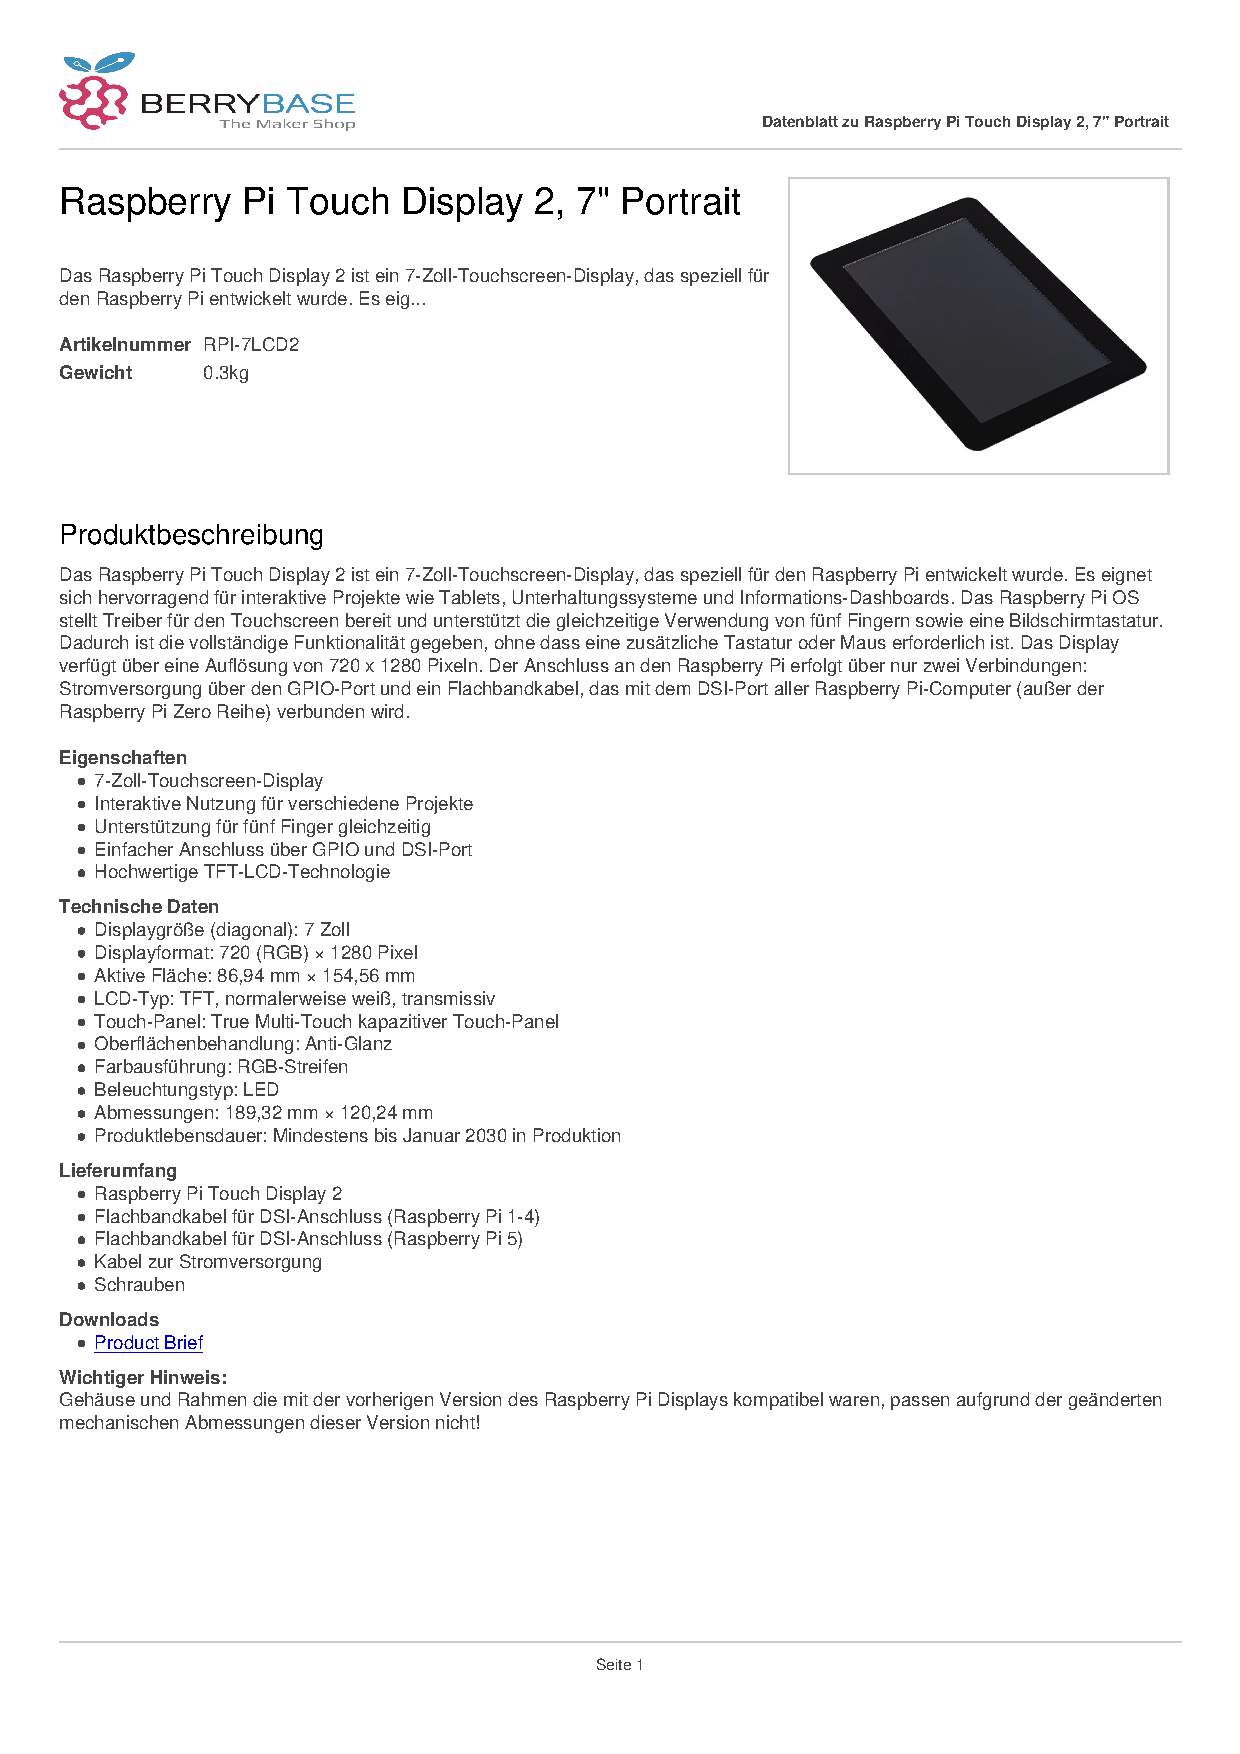
\includepdf[pages=1,scale=0.7,pagecommand={\subsection{Eingefügte PDF-Seite 1}}]{Raspberry_Display.pdf}
% pages=1 = nur erste Seite einfügen
% scale=0.8 = auf 80% skalieren
% pagecommand={} = führt Befehle auf der eingefügten Seite aus

% Kommentar: Würde Seiten 1-3 einfügen 
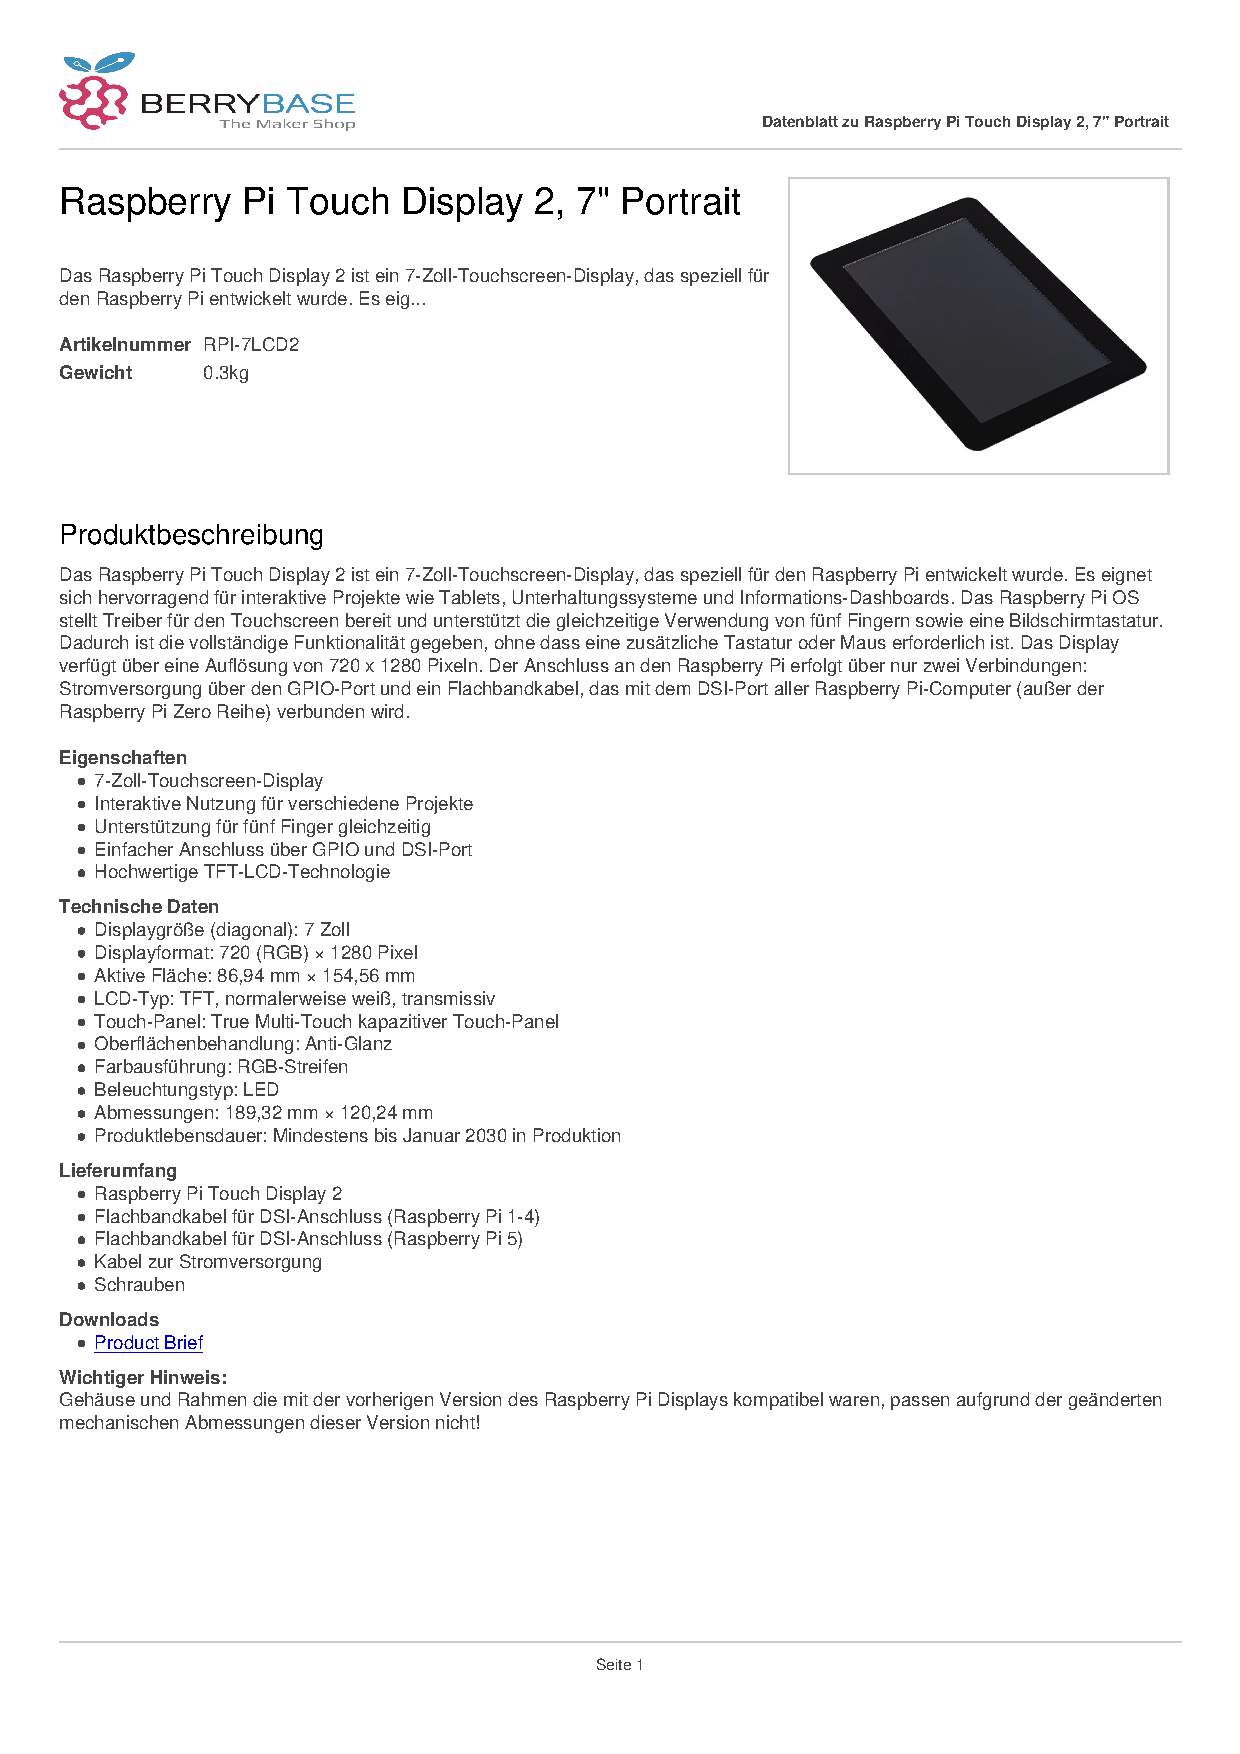
\includepdf[pages=1-3,scale=0.7,pagecommand=\subsection{Mehrere PDF-Seiten}]{Raspberry_Display.pdf}
% pages=1-3 = Seiten 1 bis 3
% pages=- = alle Seiten
% pages={1,3,5} = nur Seiten 1, 3 und 5

% =====================================================================
\subsection{Fortgeschrittene Techniken}
% Spezielle Tricks und weniger bekannte Funktionen
% =====================================================================

\subsubsection{Abbildungen ohne Nummerierung}
\begin{figure}[H]
  \centering
  
\includegraphics[width=0.5\textwidth]{BMW.jpg}
  \caption*{Unnummerierte Bildunterschrift (mit caption*).}
  % caption* (mit Stern) unterdrückt die Nummerierung
  % Abbildung erscheint NICHT im Abbildungsverzeichnis
  % Nützlich für dekorative Bilder ohne wissenschaftlichen Bezug
\end{figure}

\subsubsection{Eigenes Abbildungsverzeichnis-Format}
\begin{figure}[H]
  \centering
  
\includegraphics[width=0.5\textwidth]{Mercedes.jpg}
  \caption{Standard-Bildunterschrift mit Nummer.}
  % Normale Caption mit automatischer Nummerierung
  % Erscheint im \listoffigures
  \label{fig:standard-nummer}
\end{figure}

\subsubsection{Abbildung mit mehreren Labels}
\begin{figure}[H]
  \centering
  
\includegraphics[width=0.5\textwidth]{Porsche.jpg}
  \caption{Abbildung mit Haupt-Label.}
  \label{fig:haupt}
  % Erstes Label
  \label{fig:alternativ}
  % Zweites Label für dieselbe Abbildung
  % Beide Labels verweisen auf die gleiche Nummer
\end{figure}
Referenz auf \ref{fig:haupt} oder \ref{fig:alternativ} zeigt die gleiche Abbildung.
% Nützlich wenn man verschiedene Perspektiven auf dasselbe Bild referenzieren will

\subsubsection{Floating vs. Non-Floating}
\begin{figure}[H]
  % [H] = Non-Floating (genau hier, feste Position)
  % Abbildung bleibt exakt an dieser Stelle im Quellcode
  % Benötigt float-Paket
  % Vorteil: volle Kontrolle über Position
  % Nachteil: kann zu schlechtem Layout führen (z.B. viel Leerraum)
  \centering
  
\includegraphics[width=0.4\textwidth]{BMW.jpg}
  \caption{Non-Floating mit [H].}
\end{figure}

\begin{figure}[htbp]
  % Floating (LaTeX entscheidet die beste Position)
  % LaTeX optimiert das Layout automatisch
  % Kann auf eine andere Seite verschoben werden
  % Vorteil: professionelleres Layout, weniger Leerraum
  % Nachteil: Abbildung kann weit vom Text entfernt sein
  \centering
  
\includegraphics[width=0.4\textwidth]{Mercedes.jpg}
  \caption{Floating mit [htbp].}
\end{figure}

% =====================================================================
\subsection{Checkliste}
% Zusammenfassung wichtiger Hinweise für die Arbeit mit Abbildungen
% =====================================================================

\subsubsection{Wichtige Hinweise}

\paragraph{Dateiformat:}
\begin{itemize}
  \item \textbf{Vektorgrafiken:} PDF, EPS (ideal für Diagramme, Logos)
  \item \textbf{Rastergrafiken:} PNG (für Screenshots), JPG (für Fotos)
  \item Vermeide BMP und TIFF (große Dateien)
\end{itemize}

\paragraph{Auflösung:}
\begin{itemize}
  \item Minimum: 300 DPI für Druckqualität
  \item Web/Bildschirm: 72-150 DPI ausreichend
\end{itemize}

\paragraph{Positionierungsoptionen:}
\begin{itemize}
  \item \texttt{[H]} = Genau hier (benötigt float-Paket)
  \item \texttt{[h]} = Hier bevorzugt
  \item \texttt{[t]} = Oben auf der Seite
  \item \texttt{[b]} = Unten auf der Seite
  \item \texttt{[p]} = Eigene Seite
  \item \texttt{[!]} = Ignoriert LaTeX-Restriktionen
\end{itemize}

\paragraph{Häufige Fehler:}
\begin{itemize}
  \item Dateiendung vergessen bei \texttt{\textbackslash includegraphics}
  \item Falsche Bildpfade (verwende relative Pfade)
  \item \texttt{\textbackslash centering} vergessen
  \item Zu große Bilder ohne Skalierung
  \item Labels vergessen bei Referenzierung
\end{itemize}

\end{document}